\synctex=1
\documentclass[11pt, a4paper]{article}

%% Packages
\usepackage{subcaption}
\usepackage{amsthm}
\usepackage{amsmath}
\usepackage{amsfonts}
\usepackage{booktabs}
\usepackage{natbib}
\usepackage{hyperref}
% \usepackage{fullpage}
\usepackage{graphicx}
\usepackage{mathtools}
\usepackage{color}
\usepackage[left = 2.5cm, right = 2.5cm, bottom = 3cm, top = 2.5cm]{geometry}
\usepackage{enumitem}
\usepackage{multirow}
\usepackage{rotating}
\usepackage{calc}
\usepackage{bm}
\usepackage{pdfpages}
\usepackage{authblk}
\usepackage{dcolumn}
\usepackage{float}


\usepackage[inline]{showlabels}
\renewcommand{\showlabelfont}{\small\tt\color{red}}

%% Commands 
\newcommand*{\bb}{\boldsymbol}
\newcommand{\IK}[1]{{\noindent \color{blue} \bf \#IK: #1}}
\newcommand{\PS}[1]{{\noindent \color{red} \bf \#PS: #1}}
\newcommand{\iq}[3]{#1^{#2}_{#3}}
\newcommand{\mi}[5]{\prescript{#3}{#2}{{#1}}_{#4}^{#5}}
\newcommand{\Q}[4]{\tilde Q_{#1}^{(#2,#3,#4)}}
\newcommand{\pQ}[4]{Q_{#1}^{(#2,#3,#4)}}
\newcommand{\Op}[1]{\ensuremath{{\mathcal{O}_p(#1)}}}
\newcommand{\op}[1]{\ensuremath{{o_p(#1)}}}


\newcommand{\vnorm}[1]{\ensuremath{{\left\| #1 \right\|}}}
\newcommand{\mnorm}[1]{{\left\vert\kern-0.25ex\left\vert\kern-0.25ex\left\vert #1 
		\right\vert\kern-0.25ex\right\vert\kern-0.25ex\right\vert}}
\newcommand{\mnorms}[1]{{\vert\kern-0.25ex\vert\kern-0.25ex\vert #1 
		\vert\kern-0.25ex\vert\kern-0.25ex\vert}}
       
%% Theorems etc
\newtheoremstyle{example}% name
{3pt} %Space above
{3pt} %Space below
{} %Body font
{0\parindent} %Indent amount 1
{\bf}
% {\scshape} %Theorem head font
{:} %Punctuation after theorem head
{.5em} %Space after theorem head 2
{} %Theorem head spec (
\newtheoremstyle{theorem}% name
{3pt} %Space above
{3pt} %Space below
{\em} %Body font
{0\parindent} %Indent amount 1
{\bf}
% {\scshape} %Theorem head font
{:} %Punctuation after theorem head
{.5em} %Space after theorem head 2
{} %Theorem head spec (

\theoremstyle{example} \newtheorem{example}{Example}[section]
\theoremstyle{theorem} \newtheorem{theorem}{Theorem}[section]
\theoremstyle{theorem }\newtheorem{proposition}{Proposition}[section]
\theoremstyle{theorem }\newtheorem{corollary}{Corollary}[section]
\newtheorem{lemma}[theorem]{Lemma}

\renewcommand{\thesection}{S\arabic{section}}
\renewcommand{\theequation}{S\arabic{equation}}
\renewcommand{\thefigure}{S\arabic{figure}}
\renewcommand{\thetable}{S\arabic{table}}

%% Definitions
\def\sign{\mathop{\rm sign}}
\def\expect{{\mathop{\rm E}}}
\def\var{{\mathop{\rm var}}}
\def\cov{{\mathop{\rm cov}}}
\def\trace{{\mathop{\rm trace}}}
\def\det{{\mathop{\rm det}}}

\def\\bbeta{\bb{\\bbeta}}
\def\btheta{\bb{\theta}}
\def\bgamma{\bb{\gamma}}
\def\bSigma{\bb{\Sigma}}
\def\bgamma{\bb{\gamma}}
\def\by{\bb{y}}
\def\bC{\bb{C}}
\def\bY{\bb{Y}}
\def\bu{\bb{u}}
\def\bx{\bb{x}}
\def\bz{\bb{z}}
\def\b0{\bb{0}}
\def\bX{\bb{X}}
\def\bZ{\bb{Z}}
\def\bv{\bb{v}}
\def\bV{\bb{V}}
\def\bY{\bb{Y}}
\def\by{\bb{y}}
\def\bL{\bb{L}}
\def\bLt{\tilde{\bb{L}}}
\def\btnod{\bb{\theta}_0}
\def\bttilde{\tilde{\bb{\theta}}}
\def\bW{\bb{W}}
%% Title Page 
\title{Supplementary material for Maximum softly-penalized likelihood for Bernoulli-response generalized linear mixed models}
 
\author[1]{Philipp Sterzinger}
\author[1,2]{Ioannis Kosmidis}

\affil[1]{Department of Statistics, University of Warwick, Coventry, CV4 7AL, UK}
\affil[2]{The Alan Turing Institute, London, NW1 2DB, UK}

\begin{document}
	\maketitle
	
	\section{Supplementary Material}
		\label{sec:supp}
	All labels for the sections, equations, tables, figures and so on in the current document have been prefixed by ``S'' (e.g. Section \ref{sec:supp}, equation \eqref{eq:jeffrey_deriv_bound2}, etc). The supplementary material for \textit{Maximum softly-penalized likelihood for Bernoulli-response generalized linear mixed models} contains:
	\begin{enumerate}[label=\roman{*})]
		\item Proofs of Theorems 4.1-4.3 of the main text and a generalization to approximate likelihoods (Section \ref{sec:ass+res1}), 
		\item Bounds of the first and second order partial derivatives of Jeffreys prior (Section \ref{sec:jeffreys}), 
		\item The multivariate extension of the negative Huber loss penalty and a proof that our proposed penalties give interior point estimates for the Bernoulli-response GLMM (Section \ref{sec:mv_vc}),
		\item \PS{Ioannis content}  
		\item A summary of the simulation study of Section 6 of the main paper, and
		\item Further simulations on synthetic data (Section \ref{sec:simuls})
	\end{enumerate}
	This document and the R scripts and datasets to reproduce our results are available at \linebreak \url{https://github.com/psterzinger/softpen_supplementary}. All estimations have been conducted in R version 3.6.3 \citep{R} using the R-packages: 
	\begin{itemize}
		\item \texttt{blme} \citep{chung+etal:2013} version 1.0-5 
%		\item \texttt{broom.mixed} \citep{broom.mixed} version 0.2.7 
		%		\item \texttt{cowplot} \citep{cowplot} version 1.1.1 \PS{*}
%		\item \texttt{detectseparation} \citep{schumacher2021detect} version 0.2 
%		\item \texttt{dotwhisker} \citep{dotwhisker} version 0.7.4 
		%		\item \texttt{dplyr} \citep{dplyr} version 1.0.7 
%		\item \texttt{gridExtra} \citep{gridExtra} version 2.3 
%		\item \texttt{ggplot2} \citep{ggplot2} version 3.3.5
%		\item \texttt{ggrepel} \citep{ggrepel} version 0.9.1 
		%		\item \texttt{Hmisc} \citep{Hmisc} version 4.5-0  \PS{*}
%		\item \texttt{kableExtra} \citep{kableExtra} version 1.3.4 
%		\item \texttt{knitr} \citep{knitr} version 1.36 
%		\item \texttt{latex2exp} \citep{latex2exp} version 0.5.0 
		\item \texttt{lme4} \citep{bates+etal:2015} version 1.1.27.1
%		\item \texttt{MCMCglmm} \citep{MCMCglmm} version 2.32 
		\item \texttt{numDeriv} \citep{gilbert+varadhan:2019} version 2016.8.1.1
		\item \texttt{optimx} \citep{nash+varadhan:2011} version 2021.6.12
%		\item \texttt{RColorBrewer} \citep{RColorBrewer} version 1.1.2
%		\item \texttt{RCurl} \citep{RCurl} version 1.98-1.5   
%		\item \texttt{repmis} \citep{repmis} version 0.5 
%		\item \texttt{statmod} \citep{statmod} version 1.4.36
%		\item \texttt{tikzDevice} \citep{tikzDevice} version 0.12.3.1
%		\item \texttt{xtable} \citep{xtable} version 1.8-4 
	\end{itemize}
\newpage
	\section{Asymptotic properties of the MSP(A)L} \label{sec:ass+res1} 
	We recall our regularity assumptions for consistency.
	\begin{itemize}
		\item[SA0] Both $\ell(\btheta),\tilde{\ell}(\btheta)$ are differentiable, with  derivatives $S(\btheta),\tilde{S}(\btheta)$ 
		\item[SA1] $\underset{\btheta \in \Theta}{\sup} \; \vnorm{r_n^{-1} S(\btheta) - S_0(\btheta)} \overset{p}{\to}0$ for some deterministic function $S_0(\btheta)$ 
		\item[SA2] For all $\varepsilon>0$, $\underset{\btheta \in \Theta: \vnorm{\btheta-\btnod}\geq \varepsilon}{\inf} \vnorm{S_0(\btheta) }>0 = \vnorm{S_0(\btnod)}$ 
		\item[SA3] $\hat{\btheta}$ and $\bttilde$ are roots of $S(\btheta),\tilde{S}(\bttilde)$, i.e. $S(\hat{\btheta}) = \b0$ and $\tilde{S}(\bttilde) = \b0$. 
	\end{itemize}
	\begin{theorem}[Consistency]
		\label{thm:soft_pen_cons}
		Let $\delta^\infty = o_p(r_n)$, and assume that SA0-SA3 hold. Then $\bttilde \overset{p}{\to} \btnod$.  
	\end{theorem}
	\begin{proof}
		The proof is analogous to the proof of \citet[Theorem 1]{ogden:2017} and follows \citet[Theorem 5.9]{vaart:1998}. We give it here for completeness. First, let us bound $r_n^{-1}S(\bttilde)$: 
		\begin{equation}
		\label{eq:soft_pen_cons_proof_1}
		\begin{aligned}
		\vnorm{ r_n^{-1}S(\bttilde) } & = \vnorm{ r_n^{-1}\tilde{S}(\bttilde) + r_n^{-1}(S(\bttilde)-\tilde{S}(\bttilde)) } \\
		&= \vnorm{ \b0 -r_n^{-1}\nabla P(\bttilde) } \\
		&= o_p(1)
		\end{aligned}
		\end{equation}
		where the second equality follows from the definition of $\tilde{\ell}(\btheta) = \ell(\btheta) + P(\btheta)$ and SA3. The last equality follows from the assumption that $\delta^\infty = o_p(r_n)$. Hence, $\bttilde$, in connection with SA0-SA2, satisfies the conditions of Theorem 5.9 in \cite{vaart:1998}, which guarantees consistency. In particular, by \eqref{eq:soft_pen_cons_proof_1}, $\| r_n^{-1}{S}(\bttilde) \| =   o_p(1)$ so that adding $\| S_0(\bttilde)\|$ to both sides of this equation and rearranging yields 
		\begin{equation}
		\label{eq:soft_pen_cons_proof_2}
		\begin{aligned}
		\vnorm{S_0(\bttilde)}&=   \vnorm{S_0(\bttilde)}-\vnorm{r_n^{-1}{S}(\bttilde)} + o_p(1) \\ 
		&\leq \underset{\btheta \in \Theta}{\sup} \vnorm{r_n^{-1}{S}(\btheta)-S_0(\btheta) } + o_p(1)  \\ 
		&= o_p(1)	
		\end{aligned}
		\end{equation}
		where the second line follows from the reverse triangle inequality and the  third from \eqref{eq:soft_pen_cons_proof_1} and SA1. Finally note that SA2 implies that for any $\varepsilon>0$, there is a number $\eta$ such that $\vnorm{S_0(\btheta)}>\eta$ for any $\btheta: \vnorm{\btheta-\btnod} \geq \varepsilon$. Hence, for any $\varepsilon>0$, the event $\vnorm{\bttilde-\btnod}\geq \varepsilon$ is implied by the event $\vnorm{S_0(\bttilde)}>\eta$, however, this was seen to converge to zero in probability in \eqref{eq:soft_pen_cons_proof_2}.
	\end{proof}
	
	The proof of asymptotic normality follows the proof of \citet[Theorem 2]{ogden:2017}, with the notation adapted to the soft penalization framework. Let us restate our assumptions for asymptotic normality. 
	\begin{itemize} 
		\item[SA4] Both $\ell(\btheta),\tilde{\ell}(\btheta)$ are three times differentiable
		\item[SA5] $\underset{\btheta \in \Theta}{\sup}\; \mnorm{ r_n^{-1}J(\btheta) -I(\btheta) } \overset{p}{\to} 0$ for some positive definite, nonrandom, $\mathcal{O}(1)$ matrix $I(\btheta)$, that is continuous in $\btheta$ in a neighbourhood around $\btnod$
		\item[SA6] $r_n^{1/2}(\hat\btheta-\btnod) \overset{d}{\to} \text{N}(0,I(\btnod)^{-1})$
		\item[SA7] $\bttilde$ is consistent for $\btnod$
	\end{itemize}
	
	The following Lemma, which is an adaptation of Lemma 1 in \citet{ogden:2017}, serves to relax the stochastic order requirement of $\nabla P(\btheta)$ around $\btnod$ to achieve asymptotic normality. 
	\begin{lemma}
		\label{lemma:ogden}
		Assume that SA3, SA4, SA5 and SA7 hold. Further suppose that $\delta^\infty = o_p(r_n)$ and that there is a $t>0$ such that $\delta^{\infty}(B_t(\btnod)) = o_p(a_n)$ for some nonnegative sequence $a_n$ indexed by $n$. Then $\bttilde-\hat{\btheta}=o_p(r_n^{-1}a_n)$. 
	\end{lemma}
	\begin{proof}
		The proof is similar to \citet[Lemma 1]{ogden:2017}.
		A first order Taylor expansion of $S(\btheta)$ around $\hat{ \btheta}$ yields 
		\begin{equation}
		\label{eq:lemma_ogden_proof_1}
		\begin{aligned}
		r_n^{-1}S(\btheta) = r_n^{-1}S(\hat{\btheta}) + r_n^{-1}\nabla S(\btheta) \big|_{\btheta = \btheta^*} (\btheta - \hat{\btheta}) 
		= -J(\btheta^*) (\btheta-\hat{\btheta})
		\end{aligned}
		\end{equation}
		where $\btheta^*$ lies between $\hat \btheta$ and $\btheta$. 
		
		Now since $\nabla P(\btheta) =  \tilde{S}(\btheta) - S(\btheta)$, substituting $\bttilde$ for $\btheta$ in \eqref{eq:lemma_ogden_proof_1}, gives that
		\begin{equation}
		\label{eq:lemma_ogden_proof_2} 
		 \b0 = r_n^{-1}\tilde{S}(\bttilde) =r_n^{-1}S(\bttilde)+r_n^{-1}\nabla P(\bttilde) = -r_n^{-1}J(\btheta^*) (\bttilde-\hat{\btheta}) + r_n^{-1}\nabla P(\bttilde)
		\end{equation}
		so that
		\begin{equation}
		\label{eq:lemma_ogden_proof_3}
		\bttilde-\hat{\btheta} = [r_n^{-1}J(\btheta^*)]^{-1} r_n^{-1}\nabla P(\bttilde) 
		\end{equation}
		for some $\btheta^*$ between $\hat{\btheta}$ and $\bttilde$. Now by SA7, $\bttilde$ is consistent so that also $\btheta^*$ is consistent for $\btnod$. Hence by assumption SA5, it follows that  $[r_n^{-1}J(\btheta^*)]^{-1}$ converges in probability to $I(\btnod)^{-1}$ so that $\bttilde-\hat{\btheta} = \Op{r_n^{-1}\delta(\bttilde)} $. 
		
		Now let $A_t = \{\bttilde \in B_t(\btnod) \}$ for the $t$ such that $\delta^{\infty}(B_t(\btnod)) = o_p(a_n)$ for some nonnegative sequence $a_n$ indexed by $n$. Denote by $\bar{A}_t$, the complement to $A_t$. Then, by construction, conditional on $A_t$, $$\bttilde-\hat{\btheta}=\Op{r_n^{-1}\delta^\infty(B_t(\btnod))} =o_p(r_n^{-1}a_n) \, .$$ Moreover, since $\bttilde$ is consistent, $\Pr(A_t) \to 1$ as $n\to \infty$. Putting everything together, one gets that for any $\varepsilon>0$, 
		\begin{equation}
		\label{eq:lemma_ogden_proof_4} 
		\begin{aligned}
		\Pr\left(\|\bttilde-\btnod\| \geq \varepsilon r_n^{-1}a_n\right) & = \Pr\left(\| \bttilde-\btnod\| \geq \varepsilon r_n^{-1}a_n \mid A_t\right)\Pr(A_t)\\ &+ 
		\Pr\left(\| \bttilde-\btnod \| \geq \varepsilon r_n^{-1}a_n\mid \bar{A}_t\right)\Pr(\bar{A}_t) \\
		&\leq \Pr\left(\| \bttilde-\btnod \| \geq \varepsilon r_n^{-1}a_n \mid A_t\right) + \Pr(\bar{A}_t) \to 0, \quad n \to \infty
		\end{aligned}
		\end{equation}
		as required. 
	\end{proof}
	An immediate consequence of the Lemma and assumptions SA3-SA7 is the following theorem. 
	\begin{theorem}[Asymptotic Normality]
		\label{thm:asymp_norm_soft_pen}
		Assume that conditions SA3-SA7 hold. Let $\delta^\infty =~o_p(r_n)$ and assume there is a $t>0$ such that $\delta^{\infty}(B_t(\btnod)) = o_p(r_n^{1/2})$. Then 
		$r_n^{1/2}(\bttilde-\btnod) \overset{d}{\to} \text{N}(0,I(\btnod)^{-1})$. 
	\end{theorem}  
	\begin{proof}
		By Lemma \ref{lemma:ogden}, it holds that $\bttilde-\hat \btheta = o_p(r_n^{-1/2})$ so that $r_n^{1/2}(\bttilde-\btnod) = r_n^{1/2}(\hat{\btheta}-\btnod)+r_n^{1/2}(\bttilde-\hat{\btheta}) = r_n^{1/2}(\hat{\btheta}-\btnod) + o_p(1)$ and the result follows by SA6. 
	\end{proof}
\begin{theorem}[Hypothesis testing]\label{thm:hypo}
	Assume that conditions SA3-SA7 hold and that $\delta^\infty =~o_p(r_n)$, $\delta^\infty(B_t(\btnod)) = o_p(r_n^{1/2})$ and $\gamma^\infty(B_t(\btnod)) = o_p(r_n)$ for some $t>0$. Then, under $H_0: \tilde{\Lambda} -~\Lambda =~o_p(1)$.
\end{theorem}
	\begin{proof}
		We follow the proof of \citet[Theorem 3]{ogden:2017}. By definition of $\Lambda,\tilde{\Lambda}$, we have 
		\begin{equation}
			\frac{\tilde{\Lambda}-\Lambda}{2} = \{\tilde{\ell}(\bttilde) - \tilde{\ell}(\bttilde^R) \} - \{ {\ell}(\hat \btheta) - {\ell}(\hat{\btheta}^R) \}
		\end{equation}
		Adding and subtracting $\tilde{\ell}(\hat{\btheta})$ and $\tilde{\ell}(\hat{\btheta}^R)$ and rearranging yields 
		\begin{equation}\label{eq:hypo2}
			\frac{\tilde{\Lambda}-\Lambda}{2} =	\{\tilde{\ell}(\tilde{\btheta}) - \tilde{\ell}(\hat{\btheta}) \} +	\{\tilde{\ell}(\hat{\btheta}) - {\ell}(\hat{\btheta}) \} + \{\tilde{\ell}(\hat{\btheta}^R) - \tilde{\ell}(\tilde{\btheta}^R) \} + \{\ell(\hat{\btheta})^R-\tilde{\ell}(\hat{\btheta}^R) \}
		\end{equation}
		We first bound $\{\tilde{\ell}(\tilde{\btheta}) - \tilde{\ell}(\hat{\btheta}) \}$. For this, we do a second order Taylor expansion of $\tilde{\ell}(\hat{\btheta})$ around~$\bttilde$. Upon rearranging, we get that 
		\begin{equation}
			\tilde{\ell}(\tilde{\btheta}) - \tilde{\ell}(\hat{\btheta}) = -\tilde{S}(\bttilde)^\top(\hat{\btheta}-\bttilde) + \frac{1}{2} (\hat{\btheta}-\bttilde)^\top \tilde{J}(\btheta^*) (\hat{\btheta}-\bttilde) = \frac{1}{2} (\hat{\btheta}-\bttilde)^\top \tilde{J}(\btheta^*) (\hat{\btheta}-\bttilde)
		\end{equation}
		where $\btheta^*$ lies on the line segment between $\hat{\btheta}$ and $\bttilde$, i.e. $\btheta^* = \hat{\btheta} + c(\bttilde-\hat{\btheta})$, $c\in [0,1]$ and $\tilde{J}(\btheta) = - \nabla \nabla^\top \tilde{\ell}(\btheta) = J(\btheta) - \nabla \nabla^\top P(\btheta)$. We next show that $\tilde{J}(\btheta^*) = \Op{r_n}$, by establishing that $\nabla \nabla^\top P(\btheta^*)=o_p(r_n)$ and that $J(\btheta^*) = \Op{r_n}$. For this, let $A_t$ be the event that $\btheta^* \in B_t(\btnod)$ and denote by $\bar{A}_t$ its complement. Then for any $\varepsilon>0$, 
		\begin{equation}
			\begin{aligned}
				\Pr\left(\mnorms{r_n^{-1}\nabla \nabla^\top P(\btheta^*)}<\varepsilon\right) &= 	\Pr\left(\mnorms{r_n^{-1}\nabla \nabla^\top P(\btheta^*)}<\varepsilon\mid A_t \right)\Pr(A_t) \\ 
				&+ \Pr\left(\mnorms{r_n^{-1}\nabla \nabla^\top P(\btheta^*)}<\varepsilon\mid\bar{A}_t \right)\Pr(\bar{A}_t) \\ 
				&\leq 	\Pr\left(\mnorms{r_n^{-1}\nabla \nabla^\top P(\btheta^*)}<\varepsilon\mid A_t \right) + \Pr(\bar{A}_t) \to 0, \quad n \to \infty
			\end{aligned}
		\end{equation}
		where the first equality follows from the definition of conditional probabilities, and the second line from the fact that all probabilities are between zero and one. By assumption SA7, it follows that $\Pr(\bar{A}_t)$ converges to zero and by the assumption that $\gamma^\infty(B_t(\btnod)) = o_p(r_n)$, it follows that $\Pr\left(\mnorms{r_n^{-1}\nabla \nabla^\top P(\btheta^*)}<\varepsilon\mid A_t \right) \leq \Pr(r_n^{-1}\gamma^\infty(B_t(\btnod))>\varepsilon)$, which converges to zero. By a similar argument and using SA5, it holds that $J(\btheta^*) = \Op{r_n}$ so that we conclude that indeed $\tilde{J}(\btheta^*) = \Op{r_n}$. By Lemma \ref{lemma:ogden}, we know that $\hat{\btheta}-\bttilde = o_p(r_n^{-1/2})$ and thus 
		\begin{equation}
			\frac{1}{2} (\hat{\btheta}-\bttilde)^\top \tilde{J}(\btheta^*) (\hat{\btheta}-\bttilde) = o_p(1)
		\end{equation}
		Moreover, by SA3, $\tilde{S}(\bttilde)^\top(\hat{\btheta}-\bttilde) = \b0$, and therefore $	\tilde{\ell}(\tilde{\btheta}) - \tilde{\ell}(\hat{\btheta}) = o_p(1)$. A similar argument shows that under $H_0$, $\tilde{\ell}(\hat{\btheta}^R) - \tilde{\ell}(\tilde{\btheta}^R) =o_p(1)$. Hence, \eqref{eq:hypo2} becomes
		\begin{equation}
			\frac{\tilde{\Lambda}-\Lambda}{2} = P(\hat{\btheta})-P(\hat{\btheta}^R) + o_p(1)
		\end{equation}
		Now a first order Taylor expansion of $P(\hat{\btheta})$ around $\hat{\btheta}^R$ yields 
		\begin{equation}
			\frac{\tilde{\Lambda}-\Lambda}{2} = \nabla P(\btheta^*)^\top (\hat{\btheta}-\hat{\btheta}^R) + o_p(1)
		\end{equation}
		for some $\btheta^*$ on the line segment between $\hat{\btheta}$ and $\hat{\btheta}^R$. Now under $H_0$, $\hat{\btheta}-\hat{\btheta}^R = \Op{r_n^{-1/2}}$ Again, let $A_t$ be the event that $\btheta^* \in B_t(\btnod)$ and denote by $\bar{A}_t$ its complement. Then for any $\varepsilon>0$
		\begin{equation}
			\begin{aligned}
				\Pr(r_n^{-1/2}\|\nabla P(\btheta^*)  \| > \varepsilon) &\leq \Pr(r_n^{-1/2}\|\nabla P(\btheta^*)  \| > \varepsilon \mid A_t) \Pr(A_t) \\ 
				&+ \Pr(r_n^{-1/2}\|\nabla P(\btheta^*)  \| > \varepsilon \mid \bar{A}_t) \Pr(\bar{A}_t) \\ 
				& \leq \Pr(r_n^{-1/2}\|\nabla P(\btheta^*)  \| > \varepsilon \mid A_t) + \Pr(\bar{A}_t) \\ 
				& \leq \Pr( r_n^{-1/2}\delta^\infty(B_t(\btnod)>\varepsilon) + \Pr(\bar{A}_t) \to 0, \quad n \to \infty
			\end{aligned}
		\end{equation}
		so that $\nabla P(\btheta^*) = o_p(r_n^{1/2})$ and thus $\frac{\tilde{\Lambda}-\Lambda}{2} = o_p(1)$ as required. 
	\end{proof}
	
	If $\ell(\btheta)$ refers to an exact model likelihood that is unavailable, the framework of \citet{ogden:2017} readily gives conditions on the approximation error that preserve the asymptotic properties of Theorems \ref{thm:soft_pen_cons}-\ref{thm:hypo} for $\bttilde$. Let $\bar{\ell}(\btheta)$ be an approximation to $\ell(\btheta)$ and denote by $\bar{S}(\btheta)$ its score and by $\bar{J}(\btheta)$ its observed information matrix. For $S\subseteq \Theta$, let $\bar{\delta}^\infty(S) = \underset{\btheta \in S}{\sup} \; \| \bar{S}(\btheta)-S(\btheta)\|$ and $\bar{\delta}^\infty = \bar{\delta}^\infty(\Theta)$. Let $\tilde{\ell}(\btheta) = \bar{\ell}(\btheta)+P(\btheta)$ and denote by $\bttilde$ its maximizer over $\Theta$. Finally, define $\bar{\gamma}^\infty(S) = \underset{\btheta \in S}{\sup} \mnorms{J(\btheta)-\bar{J}(\btheta)}$.
	\begin{corollary}[Consistency of MSPAL estimates] \label{cor:cons}
		Assume that assumptions SA0-SA3 hold. Further assume that $\delta^\infty = o_p(r_n)$ and that $\bar{\delta}^\infty = o_p(r_n)$. Then $\bttilde \overset{p}{\to} \btnod$. 
	\end{corollary}
	\begin{proof}
		Note that since $\tilde{S}(\btheta) = S(\btheta) + (\bar{S}(\btheta)-{S}(\btheta)) + \nabla P(\btheta)$, by the assumptions of the Corollary and SA3, it follows that 
		\begin{equation}
			\b0 = r_n^{-1}\tilde{S}(\bttilde) = r_n^{-1}{S}(\bttilde) + r_n^{-1}(\bar{S}(\bttilde)-{S}(\bttilde)) + r_n^{-1}\nabla P(\bttilde)
		\end{equation}
		and thus 
		\begin{equation}
			r_n^{-1}{S}(\bttilde) = - r_n^{-1}(\bar{S}(\bttilde)-{S}(\bttilde)) - r_n^{-1}\nabla P(\bttilde) = o_p(1)
		\end{equation}
		Now the argument of Theorem \ref{thm:soft_pen_cons} can be applied from \eqref{eq:soft_pen_cons_proof_1} onwards.
	\end{proof}
	\begin{corollary}[Asymptotic normality of MSPAL estimates]\label{cor:asymp_norm}
		Assume that conditions SA3-SA7 hold. Let $\delta^\infty =   o_p(r_n),\bar{\delta}^\infty = o_p(r_n) $ and assume there is a $t>0$ such that $\delta^{\infty}(B_t(\btnod)) = o_p(r_n^{1/2}),\bar{\delta}^{\infty}(B_t(\btnod)) = o_p(r_n^{1/2})$. Then 
		$r_n^{1/2}(\bttilde-\btnod) \overset{d}{\to} \text{N}(0,I(\btnod)^{-1})$. 
	\end{corollary} 
	\begin{proof}
		Similar to the proof of Corollary \ref{cor:cons}, define a new ``penalty'' $\bar{P}(\btheta) = \{\bar{\ell}(\btheta)-\ell(\btheta)\}  + P(\btheta)$. Then by the triangle inequality, 
		\begin{equation}
			\begin{aligned}
				\| \nabla \bar{P}(\btheta) \| &= \|\{\bar{S}(\btheta)-{S}(\btheta) \} + \nabla P(\btheta) \| \\ 
				& \leq \|\bar{S}(\btheta) - {S}(\btheta) \| + \| \nabla P(\btheta) \| 
			\end{aligned}
		\end{equation}
		and therefore, 
		\begin{equation}
			\begin{aligned}
				\underset{\btheta \in \Theta}{\sup} 	\| \nabla \bar{P}(\btheta) \| & \leq \underset{\btheta \in \Theta}{\sup} \|\{\bar{S}(\btheta)-{S}(\btheta)\| &&+  \underset{\btheta \in \Theta}{\sup}\| \nabla P(\btheta) \|  &&&& = o_p(r_n) \\ 
				\underset{\btheta \in B_t(\btnod)}{\sup}	\| \nabla \bar{P}(\btheta) \| &\leq \underset{\btheta \in B_t(\btnod)}{\sup} \|\{\bar{S}(\btheta)-{S}(\btheta) \| &&+ \underset{\btheta \in B_t(\btnod)}{\sup}\| \nabla P(\btheta) \|  &&&& = o_p(r_n^{1/2}) \\ 
			\end{aligned}
		\end{equation}
		Hence, the proof of Theorem \ref{thm:asymp_norm_soft_pen} applies for $\bar{P}(\btheta)$ in place of $P(\btheta)$.
	\end{proof}
	\begin{corollary}[Hypothesis testing for of MSPAL]
		Assume that conditions SA3-SA7 hold and that $\delta^\infty = o_p(r_n), \bar{\delta}^\infty = o_p(r_n)$, $\delta^\infty(B_t(\btnod)) = o_p(r_n^{1/2})$,\linebreak $\bar{\delta}^\infty(B_t(\btnod)) = o_p(r_n^{1/2})$ and $\gamma^\infty(B_t(\btnod)) = o_p(r_n), \bar{\gamma}^\infty(B_t(\btnod)) = o_p(r_n)$ for some $t>0$. Then, under $H_0: \tilde{\Lambda} - \Lambda = o_p(1)$.
	\end{corollary}
	\begin{proof}
		Similarly to the proof of Corollary \ref{cor:asymp_norm}, define $\bar{P}(\btheta) = \{\bar{\ell}(\btheta)-\ell(\btheta)\} + P(\btheta)$. Then by virtue of the triangle inequality, and the assumptions of the Corollary, 
		\begin{equation}
			\begin{aligned}
				\underset{\sup \btheta \in \Theta}{\sup} \| \nabla \bar{P}(\btheta) \| &= o_p(r_n) \\ 
				\underset{\sup \btheta \in B_t(\btnod)}{\sup} \| \nabla \bar{P}(\btheta) \| &= o_p(r_n^{1/2}) \\
				\underset{\sup \btheta \in B_t(\btnod)}{\sup} \| \nabla \nabla^\top \bar{P}(\btheta) \| &= o_p(r_n) \\
			\end{aligned}
		\end{equation}
		Hence, the proof of Theorem \ref{thm:hypo} applies for $\bar{P}(\btheta)$ in place of $P(\btheta)$.
	\end{proof}
	\section{Bounds on the derivatives Jeffreys prior}
\label{sec:jeffreys}
In this section we give bounds on the first and second partial derivatives of the logarithm of Jeffreys invariant prior from a Bernoulli-response GLM with logistic link. We expect the derivations to be useful for similar such results under different link functions. 
 
\begin{theorem}[Bounding the partial derivative of the log of Jeffreys invariant prior]\label{thm:jeffrey_deriv_bound}
	Let $\bb X \in \Re^{n \times p}$ be a full column rank matrix, 
	$\bb W$ a diagonal matrix with entries
	$w_j=[\bb W]_{jj} =~\mu_j(\bb\beta)(1-~\mu_j(\bb\beta))$ 
	and $\text{logit}(\mu_j(\bb\beta)) = \bb x_{j}^\top \bb\beta$, $\bb\beta \in \Re^p$. Then 
	\begin{align}\label{eq:jeffrey_deriv_bound1}
	\left|\frac{\partial }{\partial  \beta_i}\log \det(\bb X^\top\bb W\bb X)\right|  &\leq p\underset{1\leq j\leq n}{\max} |x_{ji}(1-2\mu_j(\bb\beta))| \leq p\underset{1\leq j\leq n}{\max} |x_{ji}|, \quad \text{and} \\ \label{eq:jeffrey_deriv_bound2}
	\left|	\frac{\partial^2}{\partial \beta_i \partial \beta_j} \log\det (\bb X^\top \bb W \bb X)\right| &\leq  2p\underset{1\leq k \leq n}{\max} \; \left|x_{ki}\right| \underset{1\leq k \leq n}{\max} \; \left|x_{kj}\right|
\end{align}
\end{theorem}
\begin{proof}
We first consider the first partial derivative. It is noted without proof that 
\begin{equation}
\label{eq:jeffrey_deriv_proof}
\left|\frac{\partial }{\partial \beta_i}\log \textrm{det}(\bb X^\top\bb W\bb X)\right|  = \text{tr}\left( (\bb X^\top\bb W\bb X)^{-1}\bb X^\top\bb W\widetilde{\bb W}_i\bb X \right)
\end{equation}
where $\widetilde{\bb W}_i$ is a diagonal matrix with diagonal entries $\widetilde{w}^{(i)}_{j}=[\widetilde{\bb W}_i]_{jj}   = x_{ji}(1-2\mu_j(\bb\beta))$. 
Now by the cyclical property of the trace, it follows that 
\begin{equation}
\text{tr}\left( (\bb X^\top\bb W\bb X)^{-1}\bb X^\top\bb W\widetilde{\bb W}_i\bb X \right) =\text{tr}\left( \bb X(\bb X^\top\bb W\bb X)^{-1}\bb X^\top\bb W\widetilde{\bb W}_i \right)
\end{equation}
For notational brevity, denote the projection matrix $\bb X(\bb X^\top\bb W\bb X)^{-1}\bb X^\top\bb W$ by $\bb P$. Since $\widetilde{\bb W}_i$ is a diagonal matrix, one gets that 
\begin{align} \label{eq:jeffrey_first_line}
\left| \text{tr}\left( \bb X(\bb X^\top\bb W\bb X)^{-1}\bb X^\top\bb W\widetilde{\bb W}_i \right) \right| &=  \left| \sum_{j=1}^{n}\widetilde{w}_j^{(i)}[\bb P]_{jj} \right| \\ 
&\leq \sum_{j=1}^{n}\left|\widetilde{w}_j^{(i)}[\bb P]_{jj} \right| \\ 
&\leq \sum_{j=1}^{n}\left|\widetilde{w}_j^{(i)}\right|[\bb P]_{jj}  \\ 
&\leq \underset{1\leq j \leq n}{\max}\; \left|\widetilde{w}_j^{(i)}\right| \sum_{j=1}^{n}[\bb P]_{jj}  \\ 
%		&= \underset{1\leq j \leq n}{\max}\; \left|\widetilde{w}_j^{(i)}\right| \sum_{j=1}^{n}\lambda_j(\bb P)\\ 
&=p \underset{1\leq j \leq n}{\max}\; \left|\widetilde{w}_j^{(i)}\right|\\ 
&=p \underset{1\leq j \leq n}{\max}\; \left|x_{ji}(1-2\mu_j(\bb\beta))\right| \\ 
&\leq p\underset{1\leq j \leq n}{\max}\;\left|x_{ji}\right|  \label{eq:jeffrey_last_line}
\end{align}
Here the second line is due to the triangle inequality. The third line follows by positive-semi-definiteness of $\bb P$ and the well known property that the main-diagonal entries of a positive-semi-definite matrix are nonnegative. To see that $\bb P$ is positive-semi definite, note that $\bb X^\top\bb W\bb X$ is positive definite as $\bb X$ has full column rank and $\bb W$ is a diagonal matrix with positive entries. It thus follows that $(\bb X^\top\bb W\bb X)^{-1}$ is positive definite. Hence for any $\bb y \in \Re^{n}, \|\bb y\|_2\neq 0$, $\bb y^\top\bb X(\bb X^\top\bb W\bb X)^{-1}\bb X \bb y = \tilde{\bb y}^\top(\bb X^\top\bb W\bb X)^{-1} \tilde{\bb y} \geq 0$, for $\tilde{\by} = \bX \by$. Hence, as $\bb W$ is a diagonal matrix with nonnegative diagonal entries it follows that the main diagonal entries of $\bb P$, which are the elementwise product of the diagonals of $\bb X(\bb X^\top\bb W\bb X)^{-1}\bb X$ and $\bb W$ are nonnegative. The fifth line follows since $\bb P$ is an idempotent matrix of rank $p$, and the fact that the trace of an idempotent matrix equals its rank \citep[Corollary 10.2.2]{harville:1998}. The fact that $\bb P$ has rank $p$ follows from the assumption that $\bb X$ has full column rank and since $\bb W$ is invertible for any $\bb\beta \in \Re^p,\bb X\in \Re^{n \times p}$ by construction and is a standard result in linear algebra (see for example \cite{magnus+neudecker:2019}, Chapter 1.7).  The last line follows since $\mu_j(\bb\beta) = \textrm{logit}^{-1}(\bb x_j^{\top}\bb \beta) \in (0,1)$. 

Now consider the second partial derivative of $\log \det(\bb X^\top\bb W\bb X)$ with respect to $\beta_i,\beta_j$. That is, 
\begin{equation}
\begin{aligned}
\frac{\partial^2}{\partial \beta_i \partial \beta_j} \log\det (\bb X^\top\bb W \bb X) &= \frac{\partial}{\partial \beta_j} \textrm{tr}\left( \underbrace{\bb X(\bb X^\top\bb W\bb X)^{-1}\bb X^\top}_{:=\bb S}\bb W\widetilde{\bb W}_i\right) \\ 
&= \frac{\partial}{\partial \beta_j} \sum_{k=1}^{n}\bb S_{kk}w_k \widetilde{w}^{(i)}_k \\ 
&= \sum_{k=1}^{n}\left[\frac{\partial}{\partial \beta_j}\bb S_{kk}\right]w_k \widetilde{w}^{(i)}_k + \sum_{k=1}^{n}\bb S_{kk}\left[\frac{\partial}{\partial \beta_j}w_k \widetilde{w}^{(i)}_k\right]
\end{aligned}
\end{equation}

First consider $\frac{\partial}{\partial \beta_j}\bb S_{kk}$: 

\begin{equation}
\begin{aligned}
\frac{\partial}{\partial \beta_j}\bb S &= \frac{\partial}{\partial \beta_j}\bb X(\bb X^\top\bb W\bb X)^{-1}\bb X^\top \\ 
& = \bb X \left[\frac{\partial}{\partial\beta_j}(\bb X^\top\bb W\bb X)^{-1} \right]\bb X^\top\\ 
& = \bb X\left[-(\bb X^\top\bb W\bb X)^{-1}  \bb X^\top\bb W\widetilde{\bb W}_j\bb X(\bb X^\top\bb W\bb X)^{-1}\right]\bb X^\top
\end{aligned}
\end{equation}

Now letting $\bb P= \bb X(\bb X^\top\bb W\bb X)^{-1}\bb X^\top\bb W$, one gets that 

\begin{equation}
\begin{aligned}
\sum_{k=1}^{n}\left[\frac{\partial}{\partial \beta_j}\bb S_{kk}\right]w_k \widetilde{w}^{(i)}_k &= -\textrm{tr}\left(\bb X(\bb X^\top\bb W\bb X)^{-1}  \bb X^\top\bb W\widetilde{\bb W}_j\bb X(\bb X^\top\bb W\bb X)^{-1}\bb X^\top\bb W\widetilde{\bb W}_i \right) \\ 
&= - \textrm{tr}\left(\bb P\widetilde{\bb W}_j \bb P\widetilde{\bb W}_i \right)
\end{aligned}
\end{equation}

Now recall that $\textrm{logit}(\mu_k) = \bb x_k^\top \bb \beta$ and consider $\frac{\partial}{\partial \beta_j}w_k \widetilde{w}^{(i)}_k$: 

\begin{equation}
\begin{aligned}
\frac{\partial}{\partial \beta_j}w_k \widetilde{w}^{(i)}_k &= \frac{\partial}{\partial \beta_j}\mu_k(1-\mu_k)(1-2\mu_k)x_{ki} \\ 
&=\mu_k(1-\mu_k)\left[(1-2\mu_k)(1-3\mu_k)-\mu_k \right] x_{ki}x_{kj}
\end{aligned}
\end{equation}

Letting $\widetilde{\widetilde{\bb W}}_{ij}$ be a diagonal matrix with diagonal entries $[\widetilde{\widetilde{\bb W}}_{ij}]_{kk} = \left[(1-2\mu_k)(1-3\mu_k)-\mu_k \right] x_{ki}x_{kj}$, it thus follows that 

\begin{equation}
\begin{aligned}
\sum_{k=1}^{n}\bb S_{kk}\left[\frac{\partial}{\partial \beta_j}w_k \widetilde{w}^{(i)}_k\right] &= \textrm{tr}\left(\bb P\widetilde{\widetilde{\bb W}}_{ij} \right)
\end{aligned}
\end{equation}
and therefore 

\begin{equation}
\frac{\partial^2}{\partial \beta_i \partial \beta_j} \log\det (\bb X^\top\bb W \bb X) =\textrm{tr}\left(\bb P\widetilde{\widetilde{\bb W}}_{ij} \right) - \textrm{tr}\left(\bb P\widetilde{\bb W}_j \bb P\widetilde{\bb W}_i \right)
\end{equation}

Towards bounding these expressions, note that by similar arguments to \eqref{eq:jeffrey_first_line}-\eqref{eq:jeffrey_last_line}, it holds that 

\begin{equation}
\left|\textrm{tr}\left(\bb P\widetilde{\widetilde{\bb W}}_{ij} \right) \right| \leq p \underset{1\leq k\leq n}{\max} \; |\left[(1-2\mu_k)(1-3\mu_k)-\mu_k \right] x_{ki}x_{kj}| \leq p\underset{1\leq k\leq n}{\max} \; |x_{ki}x_{kj}|
\end{equation}
where the last inequality follows since $(1-2\mu_k)(1-3\mu_k)-\mu_k \in [-\frac{1}{2},1]$. 

Now towards bounding $\textrm{tr}\left(\bb P\widetilde{\bb W}_j \bb P\widetilde{\bb W}_i \right)$, we make the following observations. 

\begin{equation}
\begin{aligned}
\textrm{tr}\left(\bb P\widetilde{\bb W}_j \bb P\widetilde{\bb W}_i \right) &= \sum_{k=1}^{n} \left[\bb P\widetilde{\bb W}_j\bb P\widetilde{\bb W}_i\right]_{kk}\\ 
&= \sum_{k=1}^{n}\sum_{l=1}^{n}\bb P_{kl}\bb P_{lk}\widetilde{w}^{(j)}_l\widetilde{w}^{(i)}_k
\end{aligned}
\end{equation}

Also note that 
\begin{equation}
\begin{aligned}
\sum_{l=1}^{n}\left| \widetilde{w}_k^{(j)}\bb P_{kl}\bb P_{lk} \right| 
&=  \sum_{l=1}^{n} \left|\widetilde{w}^{(j)}w_kw_l [\bb X(\bb X^\top\bb W\bb X)^{-1}\bb X^\top]_{lk}^2 \right| \\ 
&= \sum_{l=1}^{n} \left|\widetilde{w}^{(j)} \right|w_kw_l [\bb X(\bb X^\top\bb W\bb X)^{-1}\bb X^\top]_{lk}^2  \\ 
&= \sum_{l=1}^{n}|\widetilde{w}^{(j)}| \bb P_{kl}\bb P_{lk} \\ 
\end{aligned}
\end{equation}
Hence 
\begin{equation}
\begin{aligned}
\left|	\textrm{tr}\left(\bb P\widetilde{\bb W}_j \bb P\widetilde{\bb W}_i \right) \right| 
&= \left| \sum_{k=1}^{n}\left[\bb P\widetilde{\bb W}_j\bb P\widetilde{\bb W}_i\right]_{kk} \right| \\ 
&=\left|\sum_{k=1}^{n}\widetilde{w}^{(i)}_k\sum_{l=1}^{n}\bb P_{kl}\bb P_{lk}\widetilde{w}^{(j)}_l \right| \\ 
&\leq 	\sum_{k=1}^{n}\left|\widetilde{w}^{(i)}_k\right|\sum_{l=1}^{n}\left| \bb P_{kl}\bb P_{lk}\widetilde{w}^{(j)}_l \right| \\ 
&\leq \underset{1\leq k \leq n}{\max} \; \left|\widetilde{w}^{(i)}_k\right| \sum_{k=1}^{n}\sum_{l=1}^{n} \bb P_{kl}\bb P_{lk}\left| \widetilde{w}^{(j)}_l \right| \\ 
&=  \underset{1\leq k \leq n}{\max} \; \left|\widetilde{w}^{(i)}_k\right| \textrm{tr}\left(\bb P|\widetilde{\bb W}_{j}|\bb P \right) \\
&=  \underset{1\leq k \leq n}{\max} \; \left|\widetilde{w}^{(i)}_k\right| \textrm{tr}\left(\bb P|\widetilde{\bb W}_{j}|\right) \\
&\leq p\underset{1\leq k \leq n}{\max} \; \left|\widetilde{w}^{(i)}_k\right| \underset{1\leq k \leq n}{\max} \; \left|\widetilde{w}^{(j)}_k\right| \\ 
&= p\underset{1\leq k \leq n}{\max} \; \left|x_{ki}(1-2\mu_k)\right| \underset{1\leq k \leq n}{\max} \; \left|x_{kj}(1-2\mu_k)\right| \\ 
&\leq  p\underset{1\leq k \leq n}{\max} \; \left|x_{ki}\right| \underset{1\leq k \leq n}{\max} \; \left|x_{kj}\right| \\ 
\end{aligned}
\end{equation}

So that it follows that 
\begin{equation}
\begin{aligned}
\left|\frac{\partial^2}{\partial \beta_i \partial \beta_j} \log\det (\bb X^\top\bb W \bb X) \right|& =\left| \textrm{tr}\left(\bb P\widetilde{\widetilde{\bb W}}_{ij} \right) - \textrm{tr}\left(\bb P\widetilde{\bb W}_j \bb P\widetilde{\bb W}_i \right) \right|\\ 
&\leq \left| \textrm{tr}\left(\bb P\widetilde{\widetilde{\bb W}}_{ij} \right) \right| + \left| \textrm{tr}\left(\bb P\widetilde{\bb W}_j \bb P\widetilde{\bb W}_i \right) \right|\\ 
&\leq p\underset{1\leq k\leq n}{\max} \; |x_{ki}x_{kj}| + p\underset{1\leq k \leq n}{\max} \; \left|x_{ki}\right| \underset{1\leq k \leq n}{\max} \; \left|x_{kj}\right| \\ 
&\leq 2p\underset{1\leq k \leq n}{\max} \; \left|x_{ki}\right| \underset{1\leq k \leq n}{\max} \; \left|x_{kj}\right| \\ 
\end{aligned}
\end{equation}
This concludes the proof. 
\end{proof}	

\section{Interior point parameter estimates}
\label{sec:mv_vc}

We first show that any lower triangular matrix $\tilde{\bL}$ with finite entries and strictly positive entries on its main diagonal defines a nondegenerate variance covariance matrix $\tilde{\bSigma} = \bLt \bLt^\top$. Using this result, we show that our proposed penalty gives a nondegenerate variance components estimate and finite fixed effects estimates for a Bernoulli-response GLMM.  

\subsection{Nondegenerate variance components estimates through Huber loss penalty}

Let $\bb \Sigma \in \Re^{q \times q}$ be a real, symmetric, positive definite (variance-covariance) matrix and denote its unique lower triangular Cholesky factor by $\bb L$. Suppose we estimate $\bb L$, denote its estimate by $\tilde{\bb L}$, to obtain an estimate $\tilde{\bb \Sigma}$ of $\bb \Sigma$, based on $\tilde{\bb \Sigma} = \tilde{\bb L}\tilde{\bb L}^\top$. It is assumed that $\tilde{\bb L}$ is a real, lower triangular matrix. We say that $\tilde{\bb \Sigma}$ is degenerate if one of the following holds: 
\begin{enumerate}[label=S\arabic{*})]
	%	\setcounter{enumi}{8}
	\item $\tilde{\bb \Sigma}$ is not symmetric
	\item $\tilde{\bb \Sigma}$ is not positive definite 
	\item Some entries of $\tilde{\bb \Sigma}$ are infinite in absolute value 
	\item There is perfect estimated correlation, i.e. there exist indices $i,j: i \neq j$: $\left|\frac{\tilde{\bb \Sigma}_{ij} }{\sqrt{ \tilde{\bb \Sigma}_{ii} \tilde{\bb \Sigma}_{jj}}}\right|=1$ 
\end{enumerate}
\begin{lemma} \label{lemma:nondeg}
	Let $\tilde{\bb L} \in \Re^{q \times q}$ be real, lower triangular matrix with finite entries and strictly positive entries on its main diagonal. Then $\tilde{\bb \Sigma} = \tilde{\bb L}\tilde{\bb L}^\top$ is not degenerate. 
\end{lemma}
\begin{proof}
	S1) is trivial and follows from $\tilde{\bb \Sigma}^\top =  (\tilde{\bb L}\tilde{\bb L}^\top)^\top = \tilde{\bb L}\tilde{\bb L}^\top = \tilde{\bb \Sigma}$.
	To show that S2) cannot hold, take any $\bb x\in \Re^q$, $\bb x\neq \bb 0_q$. Then by straightforward manipulations 
	\begin{equation}
	\label{eq:chol1}
	\begin{aligned}
	\bb x^\top\tilde{\bb \Sigma}\bb x &= \bb x^\top\tilde{\bb L}\tilde{\bb L}^\top\bb x\\ 
	&= (\tilde{\bb L}^\top\bb x)^\top\tilde{\bb L}^\top\bb x \\ 
	&= \langle \bb y,\bb y\rangle, \quad \bb y=\tilde{\bb L}^\top\bb x\\
	&\geq 0
	\end{aligned}
	\end{equation}
	where $\langle\cdot,\cdot\rangle$ denotes the standard Euclidean inner product. Hence $\tilde{\bb \Sigma}$ is positive semidefinite. Suppose that there is some $\bb x \in \Re^d$ such that $\bb x^\top \bb \Sigma \bb x=0$. Then by \eqref{eq:chol1}, $\langle \bb y,\bb y \rangle = 0$ which holds if and only if $\bb y=\bb 0_d$. Now since $\tilde{\bb L}$ is lower triangular with strictly positive diagonal entries, it is full rank. To see this, assume that $\tilde{\bb L}\bb x=\bb 0_d$ and note that $[\tilde{\bb L}\bb x]_1 = l_{11}x_1$. Since $\tilde{l}_{11}>0$, it must be that $x_1=0$. Now $[\tilde{\bb L}\bb x]_2 = \tilde{l}_{21}x_1+\tilde{l}_{22}x_2$. Since $x_1=0$ and $\tilde{l}_{22}>0$ it must again hold that $x_2=0$ and by induction $\bb x=\bb 0_d$ so that $\tilde{\bb L}$ is full rank. But then $\bb y = \tilde{\bb L}\bb x=\bb 0_d$ implies that $\bb x = \bb 0_d$ so that $\tilde{\bb \Sigma}$ is positive definite. 
	To prove that S3) does not hold, note that $\tilde{\bb \Sigma}_{ij} = \langle \tilde{\bb l}_i,\tilde{\bb l}_j \rangle$, where $\tilde{\bb l}_i$ is the ith row vector of $\tilde{\bb L}$. Since all elements of $\tilde{\bb l}_i,\tilde{\bb l}_j$ are finite, so is their inner product.  
	Finally, towards a contradiction, assume that S4) holds. Then there exist some indices $i,j, i \neq j$ such that 
	\begin{alignat}{2}\label{eq:chol2}
	&\qquad& 
	\left|\frac{\tilde{\bb \Sigma}_{ij} }{\sqrt{ \tilde{\bb \Sigma}_{ii} \tilde{\bb \Sigma}_{jj}}}\right|&=1 \\ 
	\iff&& |\tilde{\bb \Sigma}_{ij}| &= \sqrt{ \tilde{\bb \Sigma}_{ii} \tilde{\bb \Sigma}_{jj}} \\ 
	\iff && |\langle \tilde{\bb l}_i,\tilde{\bb l}_j\rangle| &= \|\tilde{\bb l}_i\|\|\tilde{\bb l}_j\|
	\end{alignat}
	where $\|\bb x\|= \sqrt{\langle\bb x ,\bb x\rangle}$ is the induced inner product norm. It follows from the Cauchy-Schwarz inequality that the equality in the last line of \eqref{eq:chol2} holds if and only if $\tilde{\bb l}_i,\tilde{\bb l}_j$ are linearly dependent. Since $\tilde{\bb L}$ is lower triangular, this is only possible if $\tilde{\bb l}_i,\tilde{\bb l}_j$ have zeroes in the same positions. But since all diagonal entries of $\tilde{\bb L}$ are strictly positive, this is not possible. Hence S4) cannot hold. 
\end{proof}

\subsection{Interior point parameter estimates for Bernoulli-response GLMMS}

\begin{theorem}[Interior point estimates]\label{thm:int_point}
	Let $\ell(\bb \theta)$ be the log-likelihood of a Bernoulli response GLMM, where $\bb \theta = (\bb \beta,  \bb L  )$ and $\bb L$ is the Cholesky factor of the variance components matrix $\bSigma$. Let 
	\begin{equation}
	\label{eq:pen_max}
	\tilde\btheta = (\tilde{\bb \beta},\tilde{\bb L}) = \arg\max_{\btheta \in \Theta} \{\ell(\btheta) + P^\textit{FE}(\bb \beta) + P^\textit{MVRE}(\bL) \} \, ,
	\end{equation}
	be the maximizer of the penalized model log-likelihood, with 
	\begin{equation}
	\label{eq:MVRE_pen} 
	P^\textit{MVRE}(\bL) = \sum_{i=1}^{N_q}P^\textit{RE}(\log(l_{ii})) + \sum_{i<j}^{q}P^\textit{RE}(l_{ij}),
	\end{equation}
	\begin{equation}
	\label{eq:RE_pen} 
	P^\textit{RE}(x) \propto \begin{cases}
	-\frac{1}{2} \{x \}^2, & \text{if } |x|\leq 1 \\ 
	- |x| + \frac{1}{2}, & \text{otherwise}
	\end{cases}  ,
	\end{equation}
	and
	\begin{equation} \label{eq:FE_pen}
		P^\textit{FE}(\bb \beta) \propto \log \det(\bX^\top\bW \bX) \, .
	\end{equation}
	Then, if $\bttilde$ exists, $\tilde{\bb \Sigma} = \tilde{\bb L} \tilde{\bb L}^\top$ is nondegenerate and all components of $\tilde{\bb \beta}$ are finite whenever there is a $\bb \theta$ in the interior of $\Theta$ such that $\ell(\bb \theta) >-\infty$.
\end{theorem}
\begin{proof}
	We first note that both penalties $P^\textit{FE}(\bb \beta)$ and $P^\textit{MVRE}(\bb L)$ as well as the log-likelihood $\ell(\bb \theta)$ are bounded from above. From \eqref{eq:RE_pen} it is immediate that \eqref{eq:MVRE_pen} is bounded from above by zero (for $\bb L= {\bb I}_q$, where ${\bb I}_q$ is the $q\times q$ identity matrix). Boundedness from above of $\log \det(\bX^\top \bW \bX)$ is shown in Theorem 2 of \citet{kosmidis+firth:2020}. Boundedness from above of $\ell(\bb \theta)$ follows from the observation that the integral inside the log of $\ell(\bb \theta)$ integrates a probability mass function, which always lies in $[0,1]$ with respect to a normal density, so that $\ell(\bb \theta)$ is bounded from above by zero. Next, we show that whenever $\btheta =(\bb \beta,\bSigma)$ is on the boundary of $\Theta$, then either $P^\textit{FE}(\bb \beta) = - \infty$ or $P^\textit{MVRE}(\bL) = -\infty$. For this, let $\Theta = \Theta_\textit{FE} \cup \Theta_\textit{MVRE}$, so that $\bb \beta \in \Theta_\textit{FE}$ and $\bL \in \Theta_\textit{RE}$. Then $\btheta \in \partial \Theta$ if and only if $\bb \beta \in \partial \Theta_\textit{FE} $ or $ \bL \in \partial \Theta_\textit{MVRE}$, where $\partial \Theta_\textit{FE}$ is the set of all $\bb \beta$ with at least one infinite component and $\partial \Theta_\textit{MVRE}$ the set of all lower triangular matrices with nonnegative diagonal elements with at least one infinite component or at least one zero entry on the main diagonal. \citet{kosmidis+firth:2020} show that for any path $\bb \beta(r) \in \Theta_{\textit{FE}}$ indexed by $r \in \Re$ such that $\lim\limits_{r \to \infty} \bb \beta(r) = \bb \beta^\infty$, $\bb \beta^\infty \in \partial \Theta_{\textit{FE}}$, $\lim\limits_{r \to \infty} P^{\textit{FE}}(\bb \beta(r)) = -\infty$. On the other hand, by definition of $\partial \Theta_\textit{MVRE}$ and noting that $\lim_{|x| \to \infty} P^\textit{RE}(x) = - \infty $, it follows that for any sequence of lower triangular matrices $\bL(r) \in \Theta_{\textit{MVRE}}$ such that $\lim\limits_{r \to \infty} \bL(r) = \bL^\infty$, $\bL^\infty \in \partial \Theta_{\textit{MVRE} }$, $\lim\limits_{r \to \infty} P^{\textit{MVRE}}(\bL(r)) = -\infty$. Hence for any sequence of $\btheta(r)$ such that $\lim\limits_{r \to \infty} \btheta(r) = \btheta^\infty$ for $\btheta^\infty \in~\partial \Theta$, $\lim\limits_{r \to \infty} \tilde{\ell}(\btheta(r)) = -\infty$. Now if there exists a $\btheta$ in the interior of $\Theta$ such that $\ell(\theta)>-\infty$, then $\ell(\bttilde) >-\infty$ and we conclude that $\bttilde$ cannot lie on the boundary. By Lemma \ref{lemma:nondeg}, we then conclude that $\tilde{\bSigma}$ is not degenerate. This concludes the proof.
\end{proof} 

\section{Further Simulations} \label{sec:simuls}

\subsection{Simulation 1: Extreme fixed effects}\label{sec:sim1}

This section presents a simulation that seeks to provoke degenerate fixed effects estimates through a strong dependence of the responses on the particular fixed effects -- a phenomenon known to occur in standard logistic regression \citep{albert+anderson:1984,kosmidis+firth:2020}.

For this, we simulate from a Bernoulli-response GLMM with univariate random effects and logistic link function as follows. For five clusters $i=1,\ldots,5$ and within cluster observations $j=1,\ldots,n$, $n \in \{50,100,200\}$, we draw an i.i.d. vector of fixed effects covariates $\bx_{ij} = (x_{i1},x_{i2},x_{i3},x_{i4},x_{i5})$ where $X_{i1}=1, {X}_{i2} \sim \text{N}(0,1), {X}_{i3}\sim \textrm{Ber}\left(\frac{1}{2}\right), {X}_{i4}\sim~\textrm{Ber}\left(\frac{1}{4}\right)$, and ${X}_{i5}\sim~\exp(1)$. The fixed effect covariates are drawn once and held fixed over the simulation. To control the degree of dependence of the responses on a particular fixed effect covariate, the parameter of fixed effects is set as $\bb \beta=(1,-0.5,\lambda,0.25,-1)$, where $\lambda$ takes integer values from $-10$ to $10$. For each specification of $n$, $\lambda$, we draw 100 samples from the model 
\begin{equation}
	\begin{aligned}
		\label{eq:sim1_model} 
		Y_{ij} \mid {u}_i & \sim \text{Bernoulli}(\mu_{ij}) \quad \text{with} \quad
		g(\mu_{ij}) = \eta_{ij} = \bx_{ij}^\top \bb \beta + u_i,\\
		u_i & \sim \text{N}(0, 9)  \quad (i = 1, \ldots, 5; j = 1, \ldots, n), \quad n\in \{50,100,200\}
	\end{aligned}
\end{equation}
The random effects dispersion parameter $\sigma = 3$ was chosen as to avoid estimation issues associated with small random effects. We estimate the parameters using our proposed MSPAL with the penalties given in Section 5 of the main text, MAL and \texttt{bglmer}  from the \texttt{blme} R package \citep{chung+etal:2013} with a normal and t prior for the fixed effects and a gamma prior for the random effects variance. We approximate the log-likelihood with a 20-point adaptive Gauss-Hermite quadrature approximation. For MAL and MSPAL, we optimize the approximate log-likelihood using the optimization methods ``CG'', ``BFGS'', ``nlminb'' and ``L-BFGS-B'' from the \texttt{optimx} R package \citep{nash+varadhan:2011} and report the best fit. Both \texttt{bglmer} specifications use the default \texttt{bglmer} optimization settings. 

Table \ref{tab:sim1} shows the number of estimates per specification which resulted in an degenerate parameter estimate. We considered an estimate degenerate, if it is larger than $50$ in absolute value, the gradient is larger than $0.001$ in absolute value, or if the estimated asymptotic standard errors are larger than $40$. Figure \ref{fig:sim1} shows the dispersion of the estimates ${\beta}_3$ around the true value (indicated by dashed horizontal line) per specification for all estimation methods. For presentability, the y-axis has been cropped to omit overly extreme estimates. For the MAL, 672 estimates are cropped, while  for \texttt{bglmer}(n), one estimation is not shown due to failed estimation (NaN output). Note that the boxplots for the MAL do not depict the empirical distribution of the MAL estimate of $\beta_3$ over different samples as theoretically infinite estimates assume finite values in estimation due to numerical precision limitations and resulting premature declaration of convergence. We see from Table \ref{tab:sim1} that the MSPAL gives the most stable parameter estimation, with one out of 6000 samples exhibiting estimation issues due to failed convergence. The MAL on the other hand becomes highly problematic for large values of $\beta_3$ and even returns degenerate estimates for moderate values of $\beta_3$ with non-negligible frequency. The \texttt{bglmer} estimates, even though they penalize fixed effects more harshly, as can be seen by the shrinkage-induced bias of the \texttt{bglmer} estimates of $\beta_3$ in Figure \ref{fig:sim1}, they encounter estimation issues substantially more often than the MSPAL estimates. 
\begin{figure}[H]
	\begin{center}
		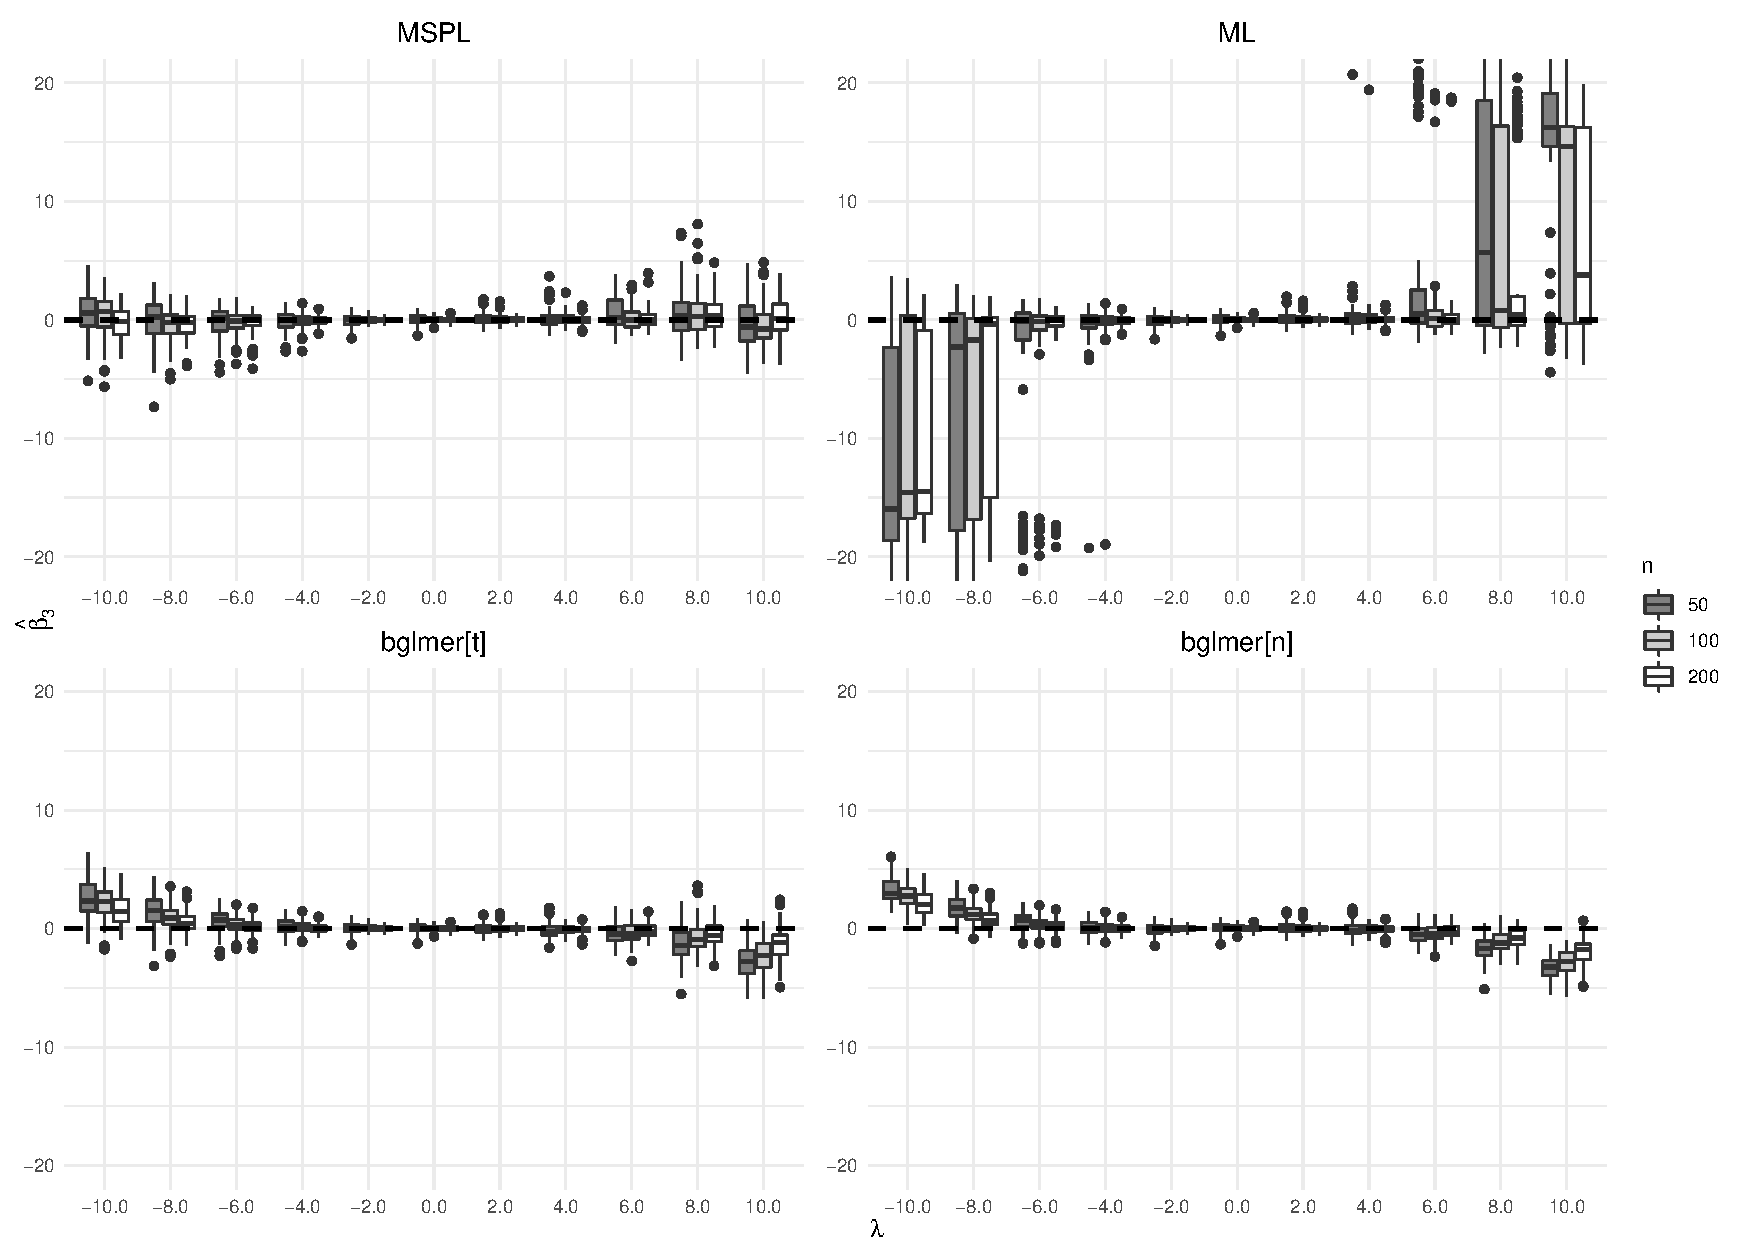
\includegraphics[width=\textwidth]{Figures/sim1.pdf}
	\end{center}
	\caption{Centered estimation output of $\hat{\beta}_3-\beta_3$ from Simulation \hyperref[sec:sim1]{1}}
	\label{fig:sim1}
\end{figure}
\begin{table}[ht]
	\centering
	\caption{Percentage of degenerate estimates from Simulation \hyperref[sec:sim1]{1}} 
	\label{tab:sim1}
	\begin{tabular}{rlccccccccccc}
	\toprule
	&& \multicolumn{11}{c}{$\lambda$} \\
	\cmidrule{3-13} 
	 &  & -10 & -8 & -6 & -4 & -2 & 0 & 2 & 4 & 6 & 8 & 10 \\ 
	\cmidrule{3-13} 
 & n=50 & 0 & 0 & 0 & 0 & 0 & 0 & 0 & 0 & 0 & 0 & 0 \\ 
MSPAL & n=100 & 0 & 0 & 0 & 0 & 0 & 0 & 0 & 0 & 0 & \textbf{1} & 0 \\ 
& n=200 & 0 & 0 & 0 & 0 & 0 & 0 & 0 & 0 & 0 & 0 & 0 \\ \cmidrule{3-13} 
& n=50 & \textbf{73} & \textbf{46} & \textbf{16} & \textbf{2} & 0 & 0 & 0 & \textbf{1} & \textbf{15} & \textbf{49} & \textbf{80} \\ 
MAL & n=100 & \textbf{63} & \textbf{45} & \textbf{10} & \textbf{1} & 0 & 0 & 0 & \textbf{1} & \textbf{5} & \textbf{31} & \textbf{61} \\ 
& n=200 & \textbf{65} & \textbf{26} & \textbf{8} & 0 & 0 & 0 & 0 & 0 & \textbf{2} & \textbf{24} & \textbf{49} \\ \cmidrule{3-13} 
& n=50 & 0 & 0 & 0 & 0 & 0 & 0 & 0 & 0 & 0 & 0 & 0 \\ 
bglmer(t) & n=100 & 0 & 0 & 0 & \textbf{1} & 0 & 0 & 0 & 0 & 0 & 0 & 0 \\ 
& n=200 & 0 & 0 & \textbf{1} & 0 & \textbf{1} & 0 & 0 & 0 & 0 & 0 & \textbf{1} \\ \cmidrule{3-13} 
& n=50 & \textbf{1} & 0 & 0 & \textbf{1} & \textbf{1} & \textbf{1} & 0 & 0 & 0 & \textbf{1} & 0 \\ 
bglmer(n) & n=100 & 0 & \textbf{1} & \textbf{1} & 0 & \textbf{2} & 0 & \textbf{1} & \textbf{1} & \textbf{1} & 0 & 0 \\ 
& n=200 & 0 & 0 & 0 & 0 & 0 & 0 & \textbf{2} & \textbf{1} & 0 & 0 & \textbf{3} \\ 
	\bottomrule
	\end{tabular}
\end{table}


\subsection{Simulation 2: Extreme random effects variance} \label{sec:sim2}
In this simulation, we seek to provoke degenerate random effects variance estimates, that is random effects variance estimates that are either zero or infinite. One of the peculiarities of Bernoulli-response (or Binomial-response) GLMMs is that there can be separation of the observations with respect to the random effects covariates. Analogously to separation in logistic regression models \citep{albert+anderson:1984}, where covariate constellations such that the responses can be separated by a hyperplane spanned by the covariate column vectors, lead to infinite parameter estimates, it is known that certain constellations of random effects covariates can lead to data separation and consequently degenerate random effects estimates (see for example \citet{sauter+held:2016} or the discussion on \url{https://stats.stackexchange.com/questions/44755}). We consider a simple simulation to provoke such data configurations by simulating from a Bernoulli-response GLMM with univariate random effects and logistic link function and vary the dependence of the responses on the grouping variable by controlling the random effects variance parameter. 

For five clusters $i=1,\ldots,5$ and within cluster observations $j=1,\ldots,n$, $n \in \{50,100,200\}$, we draw an i.i.d. vector of fixed effects covariates $\bx_{ij} = (x_{i1},x_{i2},x_{i3},x_{i4},x_{i5})$ where $X_{i1}=~1$, ${X}_{i2} \sim \text{N}(0,1), {X}_{i3}\sim \textrm{Ber}\left(\frac{1}{2}\right), {X}_{i4}\sim~\textrm{Ber}\left(\frac{1}{4}\right)$, and ${X}_{i5}\sim~\exp(1)$. The fixed effect covariates are drawn once and held fixed over the simulation. Likewise, the fixed effects $\bb \beta  =~(1,-0.5,0.5,0.25,-1)$ are held fixed over the simulation, while $\lambda = \log \sigma$ is varied  over the integer values from $-5$ to $2$. For each specification of $n$, $\lambda$, we draw 100 samples from the model 
\begin{equation}
\begin{aligned}
\label{eq:sim2_model} 
Y_{ij} \mid {u}_i & \sim \text{Bernoulli}(\mu_{ij}) \quad \text{with} \quad
g(\mu_{ij}) = \eta_{ij} = \bx_{ij}^\top \bb \beta + u_i,\\
u_i & \sim \text{N}(0, \exp (\lambda)^2 )  \quad (i = 1, \ldots, 5; j = 1, \ldots, n), \quad n\in \{50,100,200\}
\end{aligned}
\end{equation}
We estimate the parameters using our proposed MSPAL with the penalties given in Section 5 of the main text, MAL and \texttt{bglmer}  from the \texttt{blme} R package \citep{chung+etal:2013} with a normal and t prior for the fixed effects and a gamma prior for the random effects variance. We approximate the log-likelihood with a 20-point adaptive Gauss-Hermite quadrature approximation. For MAL and MSPAL, we optimize the approximate log-likelihood using the optimization methods ``CG'', ``BFGS'', ``nlminb'' and ``L-BFGS-B'' from the \texttt{optimx} R package \citep{nash+varadhan:2011} and report the best fit. Both \texttt{bglmer} specifications use the default \texttt{bglmer} optimization settings. Figure \ref{fig:sim2} shows the dispersion of the estimates for $\log \sigma$ around the true value (indicated by dashed horizontal line), for each estimation method and specification of $\lambda ,n$. For the MAL and \texttt{bglmer} estimates, these boxplots do not approximate the distribution of the maximum likelihood estimator as, owed to numerical precision limitations, parameter estimates which ought to be infinite or zero are not estimated as such so that the point masses at the boundaries of the parameter space are missing. For blgmer(t), 6 estimates are not shown and for bglmer(n), 10 estimates are not shown due to failed estimation. While both the MSPAL and \texttt{bglmer} shrink negative estimates of $\log \sigma$ towards zero, the shrinkage induced by \texttt{bglmer} is considerably stronger, as can be seen by the absolute amount of shrinkage and the smaller dispersion of the estimates. Moreover, we see that for larger values of $\log \sigma$ \texttt{bglmer} is unable to guard against infinite estimates of the random effects variance. 

Table \ref{tab:sim2} shows the number of estimates for $\log \sigma$ per specification which resulted in an degenerate random effects variance estimate. We considered an estimate degenerate, if it is larger than $\log(50)$ or smaller than $\log(0.01)$, the gradient is larger than $0.001$ in absolute value, or if the estimated asymptotic standard errors are larger than $40$. We see that MSPAL is the most stable estimation routine and that both \texttt{bglmer} and MAL exhibit estimation degeneracies frequently for both small and large values of the random effects variance. 
\begin{figure}[H]
	\begin{center}
		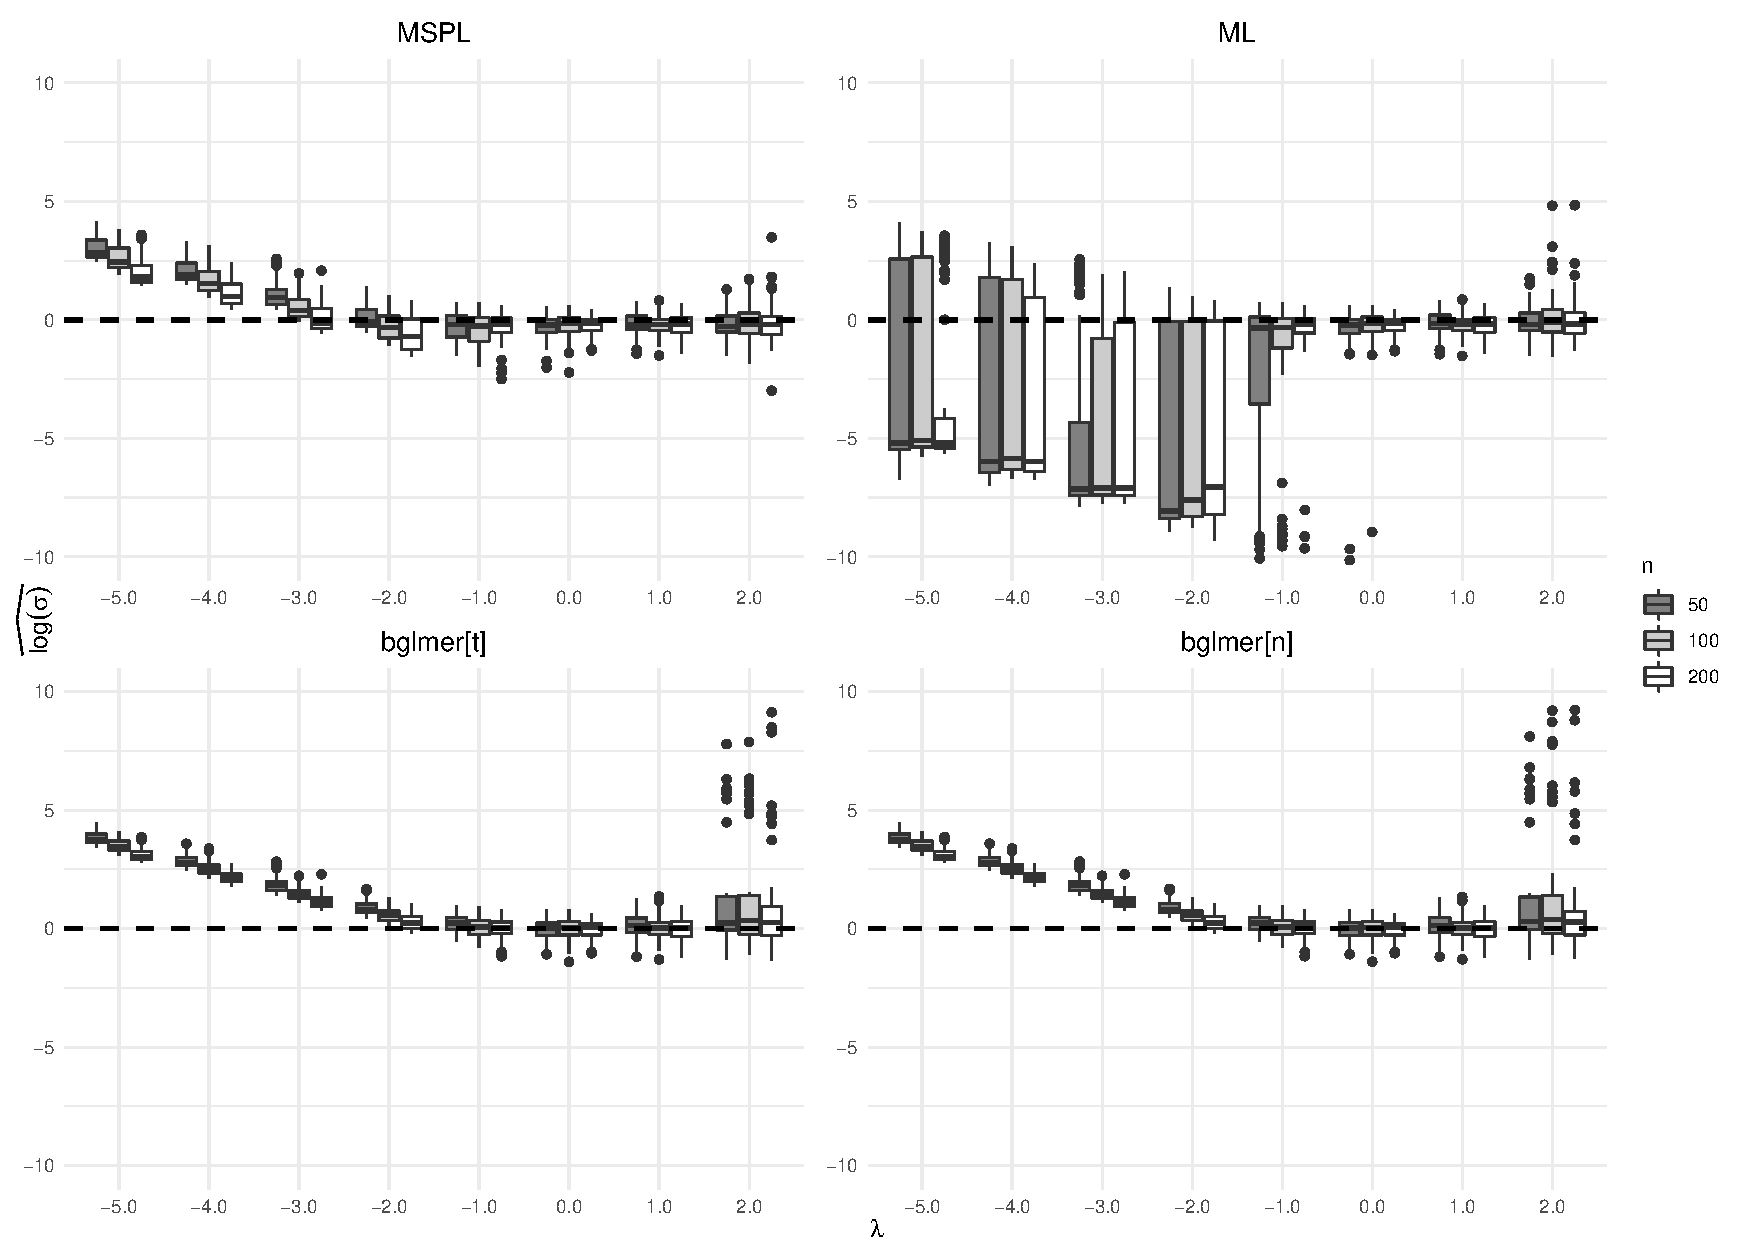
\includegraphics[width=\textwidth]{Figures/sim2.pdf}
	\end{center}
	\caption{Centered estimation output of $\widehat{\log \sigma }-\log(\sigma)$ from Simulation \hyperref[sec:sim2]{2}}
	\label{fig:sim2}
\end{figure}
\begin{table}[H]
	\centering
	\caption{Percentage of degenerate estimates from Simulation \hyperref[sec:sim2]{2}} 
	\label{tab:sim2}
		\begin{tabular}{rlcccccccc}
			\toprule
			&&\multicolumn{8}{c}{$\lambda$} \\ \cmidrule{3-10}
			&  & -5 & -4 & -3 & -2 & -1 & 0 & 1 & 2 \\ 
			\cmidrule{3-10}
			& n=50 & 0 & 0 & 0 & 0 & 0 & 0 & 0 & \textbf{1} \\ 
			MSPAL & n=100 & 0 & 0 & 0 & 0 & 0 & 0 & 0 & 0 \\ 
			& n=200 & 0 & 0 & 0 & 0 & 0 & 0 & 0 & \textbf{2} \\ \cmidrule{3-10}
			& n=50 & 0 & 0 & 0 & 0 & 0 & 0 & 0 & \textbf{12} \\ 
			bglmer(t) & n=100 & \textbf{1} & \textbf{1} & \textbf{6} & \textbf{4} & \textbf{2} & 0 & 0 & \textbf{17} \\ 
			& n=200 & \textbf{25} & \textbf{31} & \textbf{19} & \textbf{24} & \textbf{3} & 0 & 0 & \textbf{11} \\ \cmidrule{3-10}
			& n=50 & \textbf{4} & \textbf{1} & \textbf{4} & \textbf{3} & \textbf{2} & \textbf{1} & \textbf{1} & \textbf{13} \\ 
			bglmer(n) & n=100 & \textbf{21} & \textbf{19} & \textbf{14} & \textbf{14} & \textbf{11} & \textbf{2} & \textbf{1} & \textbf{20} \\ 
			& n=200 & \textbf{33} & \textbf{45} & \textbf{40} & \textbf{28} & \textbf{23} & \textbf{4} & 0 & \textbf{17} \\ \cmidrule{3-10}
			& n=50 & \textbf{73} & \textbf{70} & \textbf{76} & \textbf{70} & \textbf{25} & \textbf{2} & 0 & 0 \\ 
			MAL & n=100 & \textbf{68} & \textbf{66} & \textbf{75} & \textbf{58} & \textbf{16} & \textbf{1} & 0 & \textbf{7} \\ 
			& n=200 & \textbf{78} & \textbf{68} & \textbf{69} & \textbf{52} & \textbf{4} & 0 & 0 & \textbf{5} \\ 
			\bottomrule
		\end{tabular}
\end{table}


%\subsection{Simulation 3: Separation into clusters} \label{sec:sim3}
%One of the peculiarities of Bernoulli-response (or Binomial-response) GLMMs is that there can be separation of the observations with respect to the random effects covariates. Analogously to separation in logistic regression models \citep{albert1984existence}, where covariate constellations such that the data can be completed separated by a hyperplane spanned by the covariate vector lead to infinite parameter estimates, it is known that certain constellations of random effects covariates can lead to data separation and consequently degenerate random effects estimates (see for example \citet{sauter2016quasi} or the discussion on \url{https://stats.stackexchange.com/questions/44755}). We consider a very simple simulation to provoke such data configurations by simulating from a Bernoulli-response GLMM with only two clusters and a very large random effects variance. In particular, for clusters $i=1,2$, and within cluster observations $j=1,\ldots,n$ $n \in \{50,100,200\}$, we let the vector of fixed effects covariates $\bx_{ij}$ be an i.i.d. sample  $\bx = (x_1,x_2,x_3,x_3,x_4,x_5)$ where $X_1=1, {X}_2 \sim \text{N}(0,1), {X}_3\sim \textrm{Ber}\left(\frac{1}{2}\right), {X}_4=\textrm{Ber}\left(\frac{1}{4}\right),{X}_5\sim\exp(1)$, which is drawn once and held fixed over the simulation. The fixed effect parameters $\beta = (1,-0.5,0.5,0.25,-1)$ are held fixed while $U_i\sim \text{N}(0,\lambda^2)$ is varied via $\lambda$ which takes 20 values on the evenly spaced grid from $1$ to $10$. For each value of $n$, $\lambda$, we draw 100 samples from the model 
%\begin{equation}
%\begin{aligned}
%\label{eq:sim3_model} 
%Y_{ij} \mid {u}_i & \sim \text{Bernoulli}(\mu_{ij}) \quad \text{with} \quad
%g(\mu_{ij}) = \eta_{ij} = \bx_{ij}^\top \bb \beta + u_i,\\
%u_i & \sim \text{N}(0, \lambda^2)  \quad (i = 1,  2; j = 1, \ldots, n), \quad n\in \{50,100,200\}
%\end{aligned}
%\end{equation}
%We estimate the parameters using our proposed MSPAL with the penalties given in Section 5 of the main text, MAL and \texttt{bglmer} from the \texttt{blme} R package \citep{blme} with a 20-point adaptive Gauss-Hermite quadrature approximation to the log-likelihood. \PS{results here}
%\begin{figure}[H]
%	\begin{center}
%		\includegraphics[width=\textwidth]{Figures/sim3.pdf}
%	\end{center}
%	\caption{Centered estimates of $\widehat{\log \sigma}$ from Simulation \hyperref[sec:sim3]{3}}
%	\label{fig:sim3}
%\end{figure}
%\begin{table}[ht]
%	\centering
%	\caption{Percentage of degenerate estimates from Simulation \hyperref[sec:sim3]{3}} 
%	\label{tab:sim3}
%	\resizebox{\textwidth}{!}{%
%		\begin{tabular}{rlccccccccccccccccccccc}
%			\toprule
%			&& \multicolumn{20}{c}{$\lambda$} \\
%			\cmidrule{3-22} 
%			 &  & 0 & 0.39 & 0.67 & 0.88 & 1.06 & 1.21 & 1.35 & 1.46 & 1.57 & 1.66 & 1.75 & 1.83 & 1.9 & 1.97 & 2.03 & 2.09 & 2.15 & 2.2 & 2.25 & 2.3 \\ 
%			\cmidrule{3-22}
%			& n=50 & 0 & 0 & 0 & 0 & 0 & 0 & \textbf{4} & \textbf{4} & \textbf{10} & \textbf{4} & \textbf{7} & \textbf{12} & \textbf{8} & \textbf{12} & \textbf{18} & \textbf{17} & \textbf{10} & \textbf{13} & \textbf{19} & \textbf{22} \\ 
%			MSPAL & n=100 & 0 & 0 & 0 & 0 & \textbf{1} & \textbf{1} & \textbf{1} & \textbf{3} & \textbf{1} & \textbf{6} & \textbf{9} & \textbf{5} & \textbf{8} & \textbf{11} & \textbf{12} & \textbf{7} & \textbf{10} & \textbf{19} & \textbf{17} & \textbf{14} \\ 
%			& n=200 & 0 & 0 & 0 & 0 & 0 & 0 & 0 & \textbf{1} & \textbf{2} & \textbf{5} & \textbf{4} & \textbf{7} & \textbf{9} & \textbf{9} & \textbf{4} & \textbf{5} & \textbf{15} & \textbf{12} & \textbf{9} & \textbf{13} \\ \cmidrule{3-22}
%			& n=50 & \textbf{1} & \textbf{3} & \textbf{1} & \textbf{1} & \textbf{1} & \textbf{2} & \textbf{8} & \textbf{7} & \textbf{18} & \textbf{10} & \textbf{15} & \textbf{17} & \textbf{14} & \textbf{22} & \textbf{25} & \textbf{27} & \textbf{20} & \textbf{22} & \textbf{28} & \textbf{30} \\ 
%			MAL & n=100 & \textbf{6} & \textbf{5} & \textbf{2} & 0 & \textbf{6} & \textbf{5} & \textbf{3} & \textbf{8} & \textbf{5} & \textbf{8} & \textbf{11} & \textbf{9} & \textbf{12} & \textbf{14} & \textbf{17} & \textbf{14} & \textbf{20} & \textbf{21} & \textbf{22} & \textbf{22} \\ 
%			& n=200 & \textbf{7} & \textbf{3} & \textbf{5} & \textbf{7} & \textbf{1} & \textbf{4} & \textbf{5} & \textbf{2} & \textbf{8} & \textbf{9} & \textbf{9} & \textbf{13} & \textbf{12} & \textbf{17} & \textbf{10} & \textbf{8} & \textbf{21} & \textbf{18} & \textbf{16} & \textbf{17} \\ \cmidrule{3-22}
%			& n=50 & 0 & 0 & \textbf{1} & \textbf{2} & \textbf{1} & \textbf{6} & \textbf{9} & \textbf{13} & \textbf{19} & \textbf{20} & \textbf{20} & \textbf{21} & \textbf{29} & \textbf{30} & \textbf{29} & \textbf{28} & \textbf{32} & \textbf{33} & \textbf{44} & \textbf{47} \\ 
%			bglmer(t) & n=100 & 0 & 0 & 0 & 0 & \textbf{4} & \textbf{5} & \textbf{6} & \textbf{7} & \textbf{9} & \textbf{16} & \textbf{17} & \textbf{17} & \textbf{16} & \textbf{24} & \textbf{29} & \textbf{31} & \textbf{34} & \textbf{38} & \textbf{30} & \textbf{38} \\ 
%			& n=200 & 0 & 0 & 0 & \textbf{1} & \textbf{3} & \textbf{7} & \textbf{4} & \textbf{8} & \textbf{12} & \textbf{15} & \textbf{16} & \textbf{15} & \textbf{24} & \textbf{21} & \textbf{26} & \textbf{31} & \textbf{33} & \textbf{30} & \textbf{31} & \textbf{24} \\ \cmidrule{3-22}
%			& n=50 & 0 & 0 & \textbf{1} & \textbf{4} & \textbf{7} & \textbf{9} & \textbf{15} & \textbf{24} & \textbf{31} & \textbf{34} & \textbf{29} & \textbf{41} & \textbf{41} & \textbf{43} & \textbf{50} & \textbf{52} & \textbf{59} & \textbf{54} & \textbf{54} & \textbf{60} \\ 
%			bglmer(n) & n=100 & \textbf{1} & 0 & \textbf{1} & \textbf{2} & \textbf{6} & \textbf{10} & \textbf{11} & \textbf{21} & \textbf{15} & \textbf{27} & \textbf{35} & \textbf{35} & \textbf{38} & \textbf{42} & \textbf{49} & \textbf{45} & \textbf{45} & \textbf{52} & \textbf{45} & \textbf{49} \\ 
%			& n=200 & 0 & 0 & \textbf{1} & \textbf{1} & \textbf{7} & \textbf{8} & \textbf{9} & \textbf{16} & \textbf{21} & \textbf{26} & \textbf{31} & \textbf{36} & \textbf{30} & \textbf{43} & \textbf{44} & \textbf{49} & \textbf{54} & \textbf{41} & \textbf{43} & \textbf{50} \\ 
%			\bottomrule
%		\end{tabular}
%	}
%\end{table}

\bibliographystyle{chicago}
\bibliography{softpen}
\end{document}